% This file was created by matlab2tikz.
%
%The latest updates can be retrieved from
%  http://www.mathworks.com/matlabcentral/fileexchange/22022-matlab2tikz-matlab2tikz
%where you can also make suggestions and rate matlab2tikz.
%
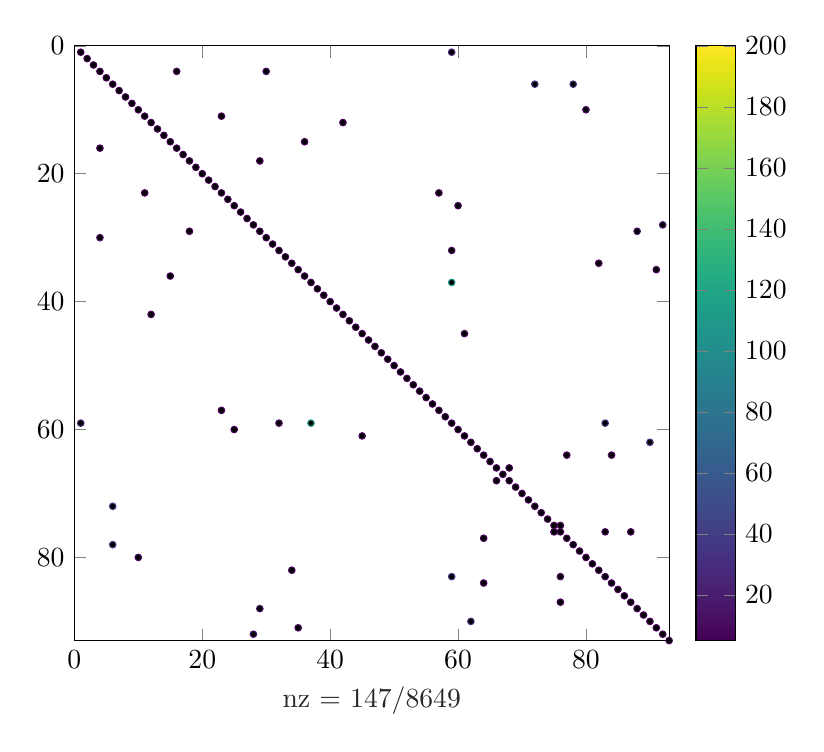
\begin{tikzpicture}

\begin{axis}[%
width=2.974in,
height=2.974in,
at={(0.269in,0.598in)},
scale only axis,
point meta min=5.04920525821867,
point meta max=200,
colormap={mymap}{[1pt] rgb(0pt)=(0.267004,0.00487433,0.329415); rgb(1pt)=(0.272651,0.0258417,0.353367); rgb(2pt)=(0.277104,0.0509074,0.376236); rgb(3pt)=(0.280353,0.0741944,0.397901); rgb(4pt)=(0.282386,0.0959463,0.418251); rgb(5pt)=(0.283199,0.116886,0.437179); rgb(6pt)=(0.282803,0.137343,0.454596); rgb(7pt)=(0.281222,0.157473,0.470434); rgb(8pt)=(0.278506,0.177342,0.484654); rgb(9pt)=(0.274723,0.196964,0.49725); rgb(10pt)=(0.269967,0.216326,0.508255); rgb(11pt)=(0.264352,0.235401,0.517732); rgb(12pt)=(0.258008,0.254159,0.52578); rgb(13pt)=(0.2511,0.272558,0.532522); rgb(14pt)=(0.243734,0.290607,0.538097); rgb(15pt)=(0.236074,0.308281,0.542652); rgb(16pt)=(0.228264,0.325578,0.546335); rgb(17pt)=(0.220425,0.342511,0.549287); rgb(18pt)=(0.212667,0.359098,0.551635); rgb(19pt)=(0.205079,0.375363,0.553493); rgb(20pt)=(0.197722,0.39134,0.554953); rgb(21pt)=(0.190631,0.407061,0.556089); rgb(22pt)=(0.183819,0.422563,0.556952); rgb(23pt)=(0.177272,0.437884,0.557576); rgb(24pt)=(0.170958,0.453061,0.557974); rgb(25pt)=(0.164833,0.468127,0.558143); rgb(26pt)=(0.158845,0.483114,0.558059); rgb(27pt)=(0.152951,0.49805,0.557685); rgb(28pt)=(0.147132,0.512957,0.556973); rgb(29pt)=(0.141402,0.527852,0.555864); rgb(30pt)=(0.135833,0.542748,0.554289); rgb(31pt)=(0.130586,0.557652,0.552188); rgb(32pt)=(0.125901,0.572563,0.549457); rgb(33pt)=(0.122165,0.587476,0.546033); rgb(34pt)=(0.119874,0.602382,0.541839); rgb(35pt)=(0.119627,0.617266,0.536803); rgb(36pt)=(0.122046,0.632107,0.530853); rgb(37pt)=(0.127667,0.646882,0.523927); rgb(38pt)=(0.136833,0.661563,0.515968); rgb(39pt)=(0.149642,0.67612,0.506924); rgb(40pt)=(0.165966,0.690519,0.49675); rgb(41pt)=(0.185537,0.704725,0.485411); rgb(42pt)=(0.20803,0.718701,0.472873); rgb(43pt)=(0.233126,0.732406,0.459103); rgb(44pt)=(0.260529,0.745802,0.444088); rgb(45pt)=(0.289997,0.758846,0.427811); rgb(46pt)=(0.321326,0.771498,0.41027); rgb(47pt)=(0.35435,0.783714,0.391454); rgb(48pt)=(0.388883,0.795453,0.371425); rgb(49pt)=(0.424885,0.806674,0.350104); rgb(50pt)=(0.462199,0.817338,0.32755); rgb(51pt)=(0.500708,0.827409,0.303804); rgb(52pt)=(0.540293,0.836858,0.278921); rgb(53pt)=(0.58082,0.845663,0.253005); rgb(54pt)=(0.622133,0.853816,0.226228); rgb(55pt)=(0.664054,0.861321,0.198883); rgb(56pt)=(0.706376,0.868206,0.171498); rgb(57pt)=(0.748863,0.874522,0.14504); rgb(58pt)=(0.791257,0.880346,0.121293); rgb(59pt)=(0.833293,0.88578,0.103327); rgb(60pt)=(0.874715,0.890945,0.0953509); rgb(61pt)=(0.915296,0.89598,0.100469); rgb(62pt)=(0.95484,0.901008,0.117874); rgb(63pt)=(0.993248,0.906157,0.143936)},
xmin=0,
xmax=93,
xlabel style={font=\color{white!15!black}},
xlabel={nz = 147/8649},
y dir=reverse,
ymin=0,
ymax=93,
axis background/.style={fill=white},
colorbar
]
\addplot[scatter, only marks, mark=*, mark size=1.1785pt, scatter src=explicit, scatter/use mapped color={mark options={}, draw=mapped color}] table[row sep=crcr, meta=color]{%
x	y	color\\
1	1	nan\\
1	59	23.9190363167076\\
2	2	nan\\
3	3	nan\\
4	4	nan\\
4	16	9.50909585257968\\
4	30	13.5127529718923\\
5	5	nan\\
6	6	nan\\
6	72	39.2911440016696\\
6	78	37.9979107834392\\
7	7	nan\\
8	8	nan\\
9	9	nan\\
10	10	nan\\
10	80	9.78139033613382\\
11	11	nan\\
11	23	6.09030700017023\\
12	12	nan\\
12	42	7.4607094126919\\
13	13	nan\\
14	14	nan\\
15	15	nan\\
15	36	6.37638798250515\\
16	4	9.50909585172252\\
16	16	nan\\
17	17	nan\\
18	18	nan\\
18	29	5.04920525821867\\
19	19	nan\\
20	20	nan\\
21	21	nan\\
22	22	nan\\
23	11	6.09030700092313\\
23	23	nan\\
23	57	6.27581072638085\\
24	24	nan\\
25	25	nan\\
25	60	6.82213207876401\\
26	26	nan\\
27	27	nan\\
28	28	nan\\
28	92	16.9495408245566\\
29	18	5.04920525861059\\
29	29	nan\\
29	88	14.7024124364251\\
30	4	13.512752972385\\
30	30	nan\\
31	31	nan\\
32	32	nan\\
32	59	11.0208651134445\\
33	33	nan\\
34	34	nan\\
34	82	5.81327047053009\\
35	35	nan\\
35	91	7.04745909470961\\
36	15	6.37638798137639\\
36	36	nan\\
37	37	nan\\
37	59	108.906483576479\\
38	38	nan\\
39	39	nan\\
40	40	nan\\
41	41	nan\\
42	12	7.46070941489722\\
42	42	nan\\
43	43	nan\\
44	44	nan\\
45	45	nan\\
45	61	11.5590592919462\\
46	46	nan\\
47	47	nan\\
48	48	nan\\
49	49	nan\\
50	50	nan\\
51	51	nan\\
52	52	nan\\
53	53	nan\\
54	54	nan\\
55	55	nan\\
56	56	nan\\
57	23	6.27581073072656\\
57	57	nan\\
58	58	nan\\
59	1	23.9190363184158\\
59	32	11.0208651166637\\
59	37	108.906483566857\\
59	59	nan\\
59	83	35.4750629162107\\
60	25	6.82213207578486\\
60	60	nan\\
61	45	11.5590592917971\\
61	61	nan\\
62	62	nan\\
62	90	30.3600793066759\\
63	63	nan\\
64	64	nan\\
64	77	7.60598221055795\\
64	84	6.11705899403339\\
65	65	nan\\
66	66	nan\\
66	68	5.89578619992027\\
67	67	nan\\
68	66	5.89578619917731\\
68	68	nan\\
69	69	nan\\
70	70	nan\\
71	71	nan\\
72	6	39.2911439977836\\
72	72	nan\\
73	73	nan\\
74	74	nan\\
75	75	nan\\
75	76	6.45352639722022\\
76	75	6.45352639788013\\
76	76	nan\\
76	83	9.4722482690906\\
76	87	5.26544750921409\\
77	64	7.60598220914878\\
77	77	nan\\
78	6	37.9979107796243\\
78	78	nan\\
79	79	nan\\
80	10	9.78139033717457\\
80	80	nan\\
81	81	nan\\
82	34	5.81327046990826\\
82	82	nan\\
83	59	35.4750629174467\\
83	76	9.47224826928785\\
83	83	nan\\
84	64	6.11705899362389\\
84	84	nan\\
85	85	nan\\
86	86	nan\\
87	76	5.26544750913584\\
87	87	nan\\
88	29	14.7024124333678\\
88	88	nan\\
89	89	nan\\
90	62	30.3600793055309\\
90	90	nan\\
91	35	7.04745909729329\\
91	91	nan\\
92	28	16.9495408218519\\
92	92	nan\\
93	93	nan\\
};
\end{axis}
\end{tikzpicture}%